%% Este formato corresponde a la versi\'onn en espa\~nol de de la Revista MMSN
%% del Departamento de Matemtica de la Universidad Tecnolgica Metropolitana, de Santiago de Chile,
%% https://mmsb.utem.cl/.
%% Esta construido usando como base el formato de acceso abierto de la IEEE.

\documentclass[eng]{MMSB-class-eng}

%%%%%%%%%%%%%%%%%%%%%%%%%%%%
% Page number where the article starts
%%%%%%%%%%%%%%%%%%%%%%%%%%%%
\setcounter{page}{1}


%%%%%%%%%%%%%%%%%%%%%%%%%%%%
% Publication title
%%%%%%%%%%%%%%%%%%%%%%%%%%%%
\title{Instructions for authors Journal Mathematical Modeling of Biological Systems\\
{\ }\\
Instrucciones para autores Revista\\Modelamiento Matem\'atico de Sistemas Biol\'ogicos}

%%%%%%%%%%%%%%%%%%%%%%%%%%%%
% Short title for the header (copy the main title if it is not too long)
%%%%%%%%%%%%%%%%%%%%%%%%%%%%
\shorttitle{Instrucciones para los autores Revista MMSB}

%%%%%%%%%%%%%%%%%%%%%%%%%%%%
% Authors
%%%%%%%%%%%%%%%%%%%%%%%%%%%%
\author[1]{Rigoberto Inostroza Basigalupo}
\author[2]{Maximiliano Buenaventura P\'erez}
\author[1,2]{Benjam\'in Gonz\'alez Leiva}

%%%%%%%%%%%%%%%%%%%%%%%%%%%%
% Author Affiliations
%%%%%%%%%%%%%%%%%%%%%%%%%%%%
\affil[1]{Departamento de Matem\'atica, Universidad Tecnol\'ogica Metropolitana, Santiago, Chile}
\affil[2]{Departamento de Ecolog\'ia, Universidad de la Naci\'on, La Paz, Bolivia}
%\affil[3]{Nombre de Departamento o Instituto, Nombre Universidad, Provincia o Estado, País}

%%%%%%%%%%%%%%%%%%%%%%%%%%%%
% Last name of the first author of the work
%%%%%%%%%%%%%%%%%%%%%%%%%%%%
\firstauthor{Inostroza Basigalupo}

%%%%%%%%%%%%%%%%%%%%%%%%%%%%
% Contact author details
%%%%%%%%%%%%%%%%%%%%%%%%%%%%
\contactauthor{Inostroza Basigalupo}
\email{Rinostroza@utem.cl} 
\mailingaddress{Las Palmeras 3360, \~Nu\~noa, Chile}
\phonenumber{+56 2 2787 7522}

%%%%%%%%%%%%%%%%%%%%%%%%%%%%
% Publication data (will be defined in the edition)
%%%%%%%%%%%%%%%%%%%%%%%%%%%%
\thisvolume{XX}
\thisnumber{XX}
\thismonth{MES}
\thisyear{20XX}
\receptiondate{dd/mm/aaaa}
\acceptancedate{dd/mm/aaaa}
\publicationdate{dd/mm/aaaa}


%%%%%%%%%%%%%%%%%%%%%%%%%%%%
% Place your particular definitions here
%%%%%%%%%%%%%%%%%%%%%%%%%%%%
\newcommand{\vect}[1]{\mathbf{#1}}

%%%%%%%%%%%%%%%%%%%%%%%%%%%%
% Start document
%%%%%%%%%%%%%%%%%%%%%%%%%%%%
\begin{document}

%%%%%%%%%%%%%%%%%%%%%%%%%%%%
% Introduzca aquí el resumen en español
%%%%%%%%%%%%%%%%%%%%%%%%%%%%
\resumen{
La Revista \emph{Modelamiento Matem\'atico de Sistemas Biol\'ogicos}, MMSB, es una publicaci\'on del grupo MatBio-UTEM, del Departamento de Matem\'atica de la Universidad Tecnol\'ogica Metropolitana, Santiago, Chile. Los autores interesados en presentar manuscrito puede usar la siguiente plantilla para preparar sus trabajos. MMSB promueve el acceso al conocimiento de manera democrática y sin fines de lucro, por lo tanto la revista no efectúa cobros por publicación a los autores ni cobros de acceso a los lectores, tampoco restringe la libre circulación de sus artículos, que no sea la debida referencia a la fuente. MMSB, busca valorizar la investigación científica producida en América Latina y el Caribe ofreciendo una vitrina para los trabajos de investigadores jóvenes de la región, sin perjuicio que es una publicación disponible a los investigadores de todos el mundo y de todas las edades.
}

%%%%%%%%%%%%%%%%%%%%%%%%%%%%
% Introduzca aquí las palabras clave en español
%%%%%%%%%%%%%%%%%%%%%%%%%%%%
\palabrasclave{
Biomatem\'atica, Biolog\'ia Matem\'atica, Ecolog\'ia Matem\'atica, Epidemiolog\'ia Matem\'atica, Biotecnolog\'ia Matem\'atica}

%%%%%%%%%%%%%%%%%%%%%%%%%%%%
% Insert here the abstract in English language
%%%%%%%%%%%%%%%%%%%%%%%%%%%%
\abstract{The Journal of \emph{Mathematical Modeling of Biological Systems}, MMSB, is a publication of the MatBio-UTEM group, of the Department of Mathematics of the Universidad Tecnológica Metropolitana, Santiago, Chile. Authors interested in submitting manuscripts can use the following template to prepare their papers. MMSB promotes access to knowledge in a democratic and non-profit manner, therefore the journal does not charge authors for publication or access charges to readers, nor does it restrict the free circulation of its articles, other than due reference to the source. MMSB seeks to value the scientific research produced in Latin America and the Caribbean by offering a showcase for the works of young researchers in the region, without prejudice that it is a publication available to researchers from all over the world and of all ages.}

%%%%%%%%%%%%%%%%%%%%%%%%%%%%
% Insert here the keywords of your work in English language
%%%%%%%%%%%%%%%%%%%%%%%%%%%%
\keywords{Biomathematics, Mathematical Biology, Mathematical Ecology, Mathematical Epidemiology, Mathematical Biotechnology}

%%%%%%%%%%%%%%%%%%%%%%%%%%%%
% Include title, authors, abstract, etc.
%%%%%%%%%%%%%%%%%%%%%%%%%%%%
\maketitle
\thispagestyle{fancy}
%\printcontactdata

%%%%%%%%%%%%%%%%%%%%%%%%%%%%
% Main body of work
%%%%%%%%%%%%%%%%%%%%%%%%%%%%
\newpage
\section{Introduction}
\primerapalabra{T}{he}% Letra capital en primera palabra
Journal of Mathematical Modeling of Biological Systems (MMSB) is an official publication of the Metropolitan Technological University of Santiago de Chile, which seeks to disseminate original works that increase the knowledge and understanding of biological systems through mathematical modeling as the main analysis tool.\\

The thematic areas include: Population Dynamics, Sustainability, Biodiversity, Epidemiology, Non-infectious Diseases, Biotechnology, Biomaterials, Neuroscience, Genetics, Genomics, Cell Biology, Physiology among other topics of biological origin that can be mathematically modeled.\\

MMSB values and promotes the use of the Spanish language in scientific dissemination but is aware that reaching a wider audience requires the use of the English language, for this reason it accepts manuscripts in either of the two options, but requires that the abstract and keywords are always in both languages. There is a \emph{template} for each language which can be downloaded from the official page of the journal \texttt{www.revistammsb.utem.cl}\\

%MMSB values ​​and promotes the use of the Spanish language in scientific dissemination but is aware that reaching a wider audience requires the use of the English language, for this reason it accepts manuscripts in either of the two options, but requires that the abstract and keywords are always in both languages. There is a \emph{template} for each language which can be downloaded from the official page of the journal \texttt{www.revistammsb.utem.cl}\\

In this example you will find indications for the good that of the formatting options, authors are recommended to follow the instructions to facilitate the good composition and reading of their manuscript. Here you will find the correct use of sections, theorems, proofs, citations and bibliography \\

All MMSB editorial policies can be consulted on the magazine's website. Queries can be sent to the email \texttt{revista.mmsb@utem.cl}


\section{The Environments}

The format of the magazine allows the following environments; Definition, Theorem, Proposition, Lemma, Corollary, Example and Note. Each of them is numbered consecutively independently. Examples of the use of these environments are shown below.\\

\begin{definition}[Ecological Niche]
 In ecology, a niche is a property that describes a species or population in an ecosystem The niche is an abstract but central concept in ecology. Although there are several definitions of niche, one of the most widely used definitions is the one that describes the niche as a multidimensional hypervolume that includes all the biotic and abiotic factors with which the organism is related.
\end{definition}


\begin{theorem}\label{teo:existencia}
Let $f(t,x):\Omega \subseteq \mathbb {R} \times \mathbb {R} ^{n}\longrightarrow \mathbb {R} ^{n}$, where $\Omega$  is a open set and $f$ is a continual and local Lipschitz fuction with respect to $x$. Then, given $(t_{0},x_{0})\in \Omega$, we can find a closed interval $I_{\alpha }=[t_{0}-\alpha ,t_{0}+\alpha ]\subset \mathbb {R} ,\alpha >0$, where there is a unique solution of the following Cauchy problem:\\
\[
 {\displaystyle {\begin{cases}x'=f(t,x)\\x(t_{0})=x_{0}\end{cases}}}
\]
It is satisfying that pairs ${\displaystyle (t,x(t))\in \Omega ,\forall t\in I_{\alpha }}$.

\end{theorem}


\begin{proposition}
Let $(x_n)$ a monotonic and bounded sequence, then it has a limit.
\end{proposition}


\begin{corollary}
Let $f:]a,b[\to\mathbb{R}$ a Lipschitz fuction. Then the differential equation 
 \[
 {\displaystyle {\begin{cases}\frac{dx}{dt}=f(x)\\x(0)=x_{0}\end{cases}}}
\]
admits a unique solution. This result follows immediately from Theorem \ref{teo:existencia}.
\end{corollary}


\begin{lemma}
 Forall pair of number $x,y\in\mathbb{R}$ we have to
 \[
  x^2+y^2\ge2xy
 \]

\end{lemma}

\begin{example}[The logistics case] A population, whose dynamics is growing logistically, can be modeled by the following differential equation
\[
 \frac{dx}{dt}=rx\left(1-\frac{x}{K}\right)
\]
where $r$ is the intrinsic growth rate of the species and $K$ is the carrying capacity of the environment.
 
\end{example}


\begin{remark}
 Exponential growth was proposed by Thomas Malthus in the book \emph{An Essay on the Principle of Population} in 1798.
\end{remark}

\section{The equations:}

As is the common usage is \LaTeX, it is possible to use both numbered and unnumbered formulas. Use numbering only in those formulas that you will cite later. To label an equation use the command \verb!\label!. To quote an equation use the command \verb!\eqref !, which automatically places the parentheses around the equation number. \\

The following commands display an equation numbered and labeled with the name \verb!ec:1!

\begin{verbatim}
\begin{equation}\label{ec:1}
  \sum_{n=1}^\infty a_nx^n=\frac{1}{x^2+1}
\end{equation}
\end{verbatim}
la que produce la ecuaci\'on
\begin{equation}\label{ec:1}
\sum_{n=1}^\infty a_nx^n=\frac{1}{x^2+1}
\end{equation}

The equation \eqref{ec:1} it will be cited in the development of the text.\\

The following commands display an unnumbered equation
\begin{verbatim}
\[
  \frac{d^2f}{dx^2}+2\frac{df}{dx}+f=0
\]
\end{verbatim}
those that produce the equation
\[
 \frac{d^2f}{dx^2}+2\frac{df}{dx}+f=0
\]

\section{The figures}

%----- Figure.
\begin{figure}[!tb] 
 \centering
 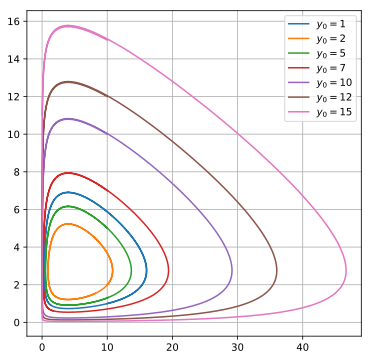
\includegraphics[width=0.8\columnwidth]{figura1} 
 \caption{Phase-space graph for the problem of predator-prey for different initial conditions of the population of predators.} \label{fig-1}
\end{figure}
%----- Fin Figure.

Figures should be included properly referenced using traditional \LaTeX\ commands, and should never be placed as individual elements within the text.\\

The figure caption or caption is automatically positioned using the environment
\begin{verbatim}
\begin{figure}[!tb]
  \centering
  \includegraphics[<options>]{<file>}
  \caption{Epígrafe} \label{<etiqueta>}
\end{figure}
\end{verbatim}

and filling in the corresponding field in \verb!\caption{<>}! (look Fig.~\ref{fig-1}). You can use files in pdf, jpg, png formats among others. Inside the field \verb![<options>]! you can adjust the size of the figure to a factor of 0.8 of the width of the column with the option \verb![width=0.8\columnwidth]!.\\

It is preferable that the figures are arranged at the beginning or at the end of the text columns, which can be achieved using the option \texttt{[!tb]}), as shown in the example in Fig \ref{fig-1}.\\

If your chart needs to be displayed using the space of the two columns use the environment \verb!\begin{figure*}!, instead of the environment \verb!\begin{figure}!, as shown in the graph in Fig.~\ref{fig-2}.

% ----- Figure two columns.
\begin{figure*}[!tb] 
 \centering
 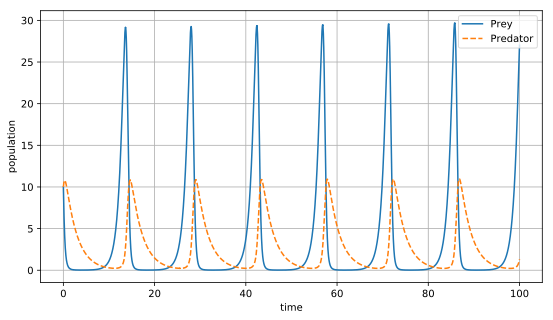
\includegraphics[width=12cm]{figura2} 
 \caption{Population dynamics baboons and cheetahs using the Lotka-Volterra equations for the problem of predotor-prey.} \label{fig-2}
\end{figure*}
% ----- End. Figure two columns.

\section{Sections and subsections}
This format allows the use of three levels of sections, section, subsection and subsubsection, with the standard \LaTeX commands. Sections and subsections are not numbered.


\section{The tables}
Avoid including tables as graphic files as much as possible, as this affects the quality of the article's composition. Therefore, always try to use the \LaTeX commands, for table use.\\

The epigraphs must be placed at the top of the table, unlike the figures, always using the command \verb!\caption!, as shown in the example in Table~\ref{tabla-1}.\\

It is preferable that the tables are located at the beginning or at the bottom of the columns. If the upper part of the column is already occupied, then occupy the lower part to avoid overlapping the two objects.\\

Avoid using text sizes smaller than 7 pt or larger than 10 pt.

\begin{table}[!b]
 \centering
  \caption{Temperature evolution for the first four states between the years 2010 - 2013}\label{tabla-1}
 {\small
 \begin{tabular}{c|ccccc}
  \hline
  \hline
  \thead{Regions \\ studieds} & \thead{2010} & \thead{2011} & \thead{2012} & \thead{2013} & \thead{2014} \\
%  \hline
  \hline
  Region 1 & $28.3$ & $28.7$ & $29.1$ & $28.9$ & $29.0$ \\

  Region 2 & $27.8$ & $28.1$ & $28.4$ & $28.2$ & $28.3$ \\
  
  Region 3 & $28.5$ & $28.7$ & $29.3$ & $29.0$ & $29.1$ \\
  
  Region 4 & $28.2$ & $28.6$ & $29.0$ & $29.0$ & $29.1$ \\
  \hline
  \hline
 \end{tabular}}
\end{table}

\section{Bibliographic standards}
Bibliographic citations, within the text, are shown in the format \emph{(Author/s, ~year)} inside parentheses. The authors appear, separated with commas and incorporating the expression \emph{et~al.} when there are three or more authors. For example, for an author \citep{Volterra1929}, twos authors \citep{GonzalezLorca1994} and three or more authors \citep{bahill1975main}.\\

This format requires the use of \texttt{Bibtex}and the package\texttt{natbib}, so the references must be included in an external file \texttt{*.bib}. In this document we used the file (\texttt{MMSM-Biblio.bib}.\\

The reference to a bibliographic citation is made with the command \verb!\citep{<etiqueta>}!,and the textual inclusion of a quote by means of \verb!\citet{<etiqueta>}!. For example, as expressed in the book of \citep{Murray2007}.\\

The following types of bibliographic references are supported.
\begin{itemize}
 \item Book: as in \citep{Murray2007}.
 \item Book chapter: as in  \citep{Jones2009}.
 \item Journal article: as in \citep{Volterra1929}.
 \item Conferences and symposia: as in \citep{BarkovaJouvet1999}.
 \item Website: as in\citep{lopez2006guia}.
 \item Technical report: as in \citep{NACA460}.
 \item Thesis or final work: as in \citep{Krause2014}.
 \item Manual or technical memory: as in\citep{Indura2010}.
 \item Other forms of communication: as in \citep{Radio2015}.
\end{itemize}

For the use of each of the bibliographic types you can edit the file \texttt{MMSMBiblio.bib} y consultar el manual de \citep{lopez2006guia}.\\

To include the bibliography use the command
\begin{verbatim}
 \insertbibliography{<archivo.bib>} 
\end{verbatim}
at the end of the manuscript.

\section{Acknowledgments}
To include acknowledgments, references to research projects, or entities
funders of the work, these should be included in the ``Acknowledgments'' section after the conclusions of the work.
Verify correctly placing the names and codes corresponding to the research projects, institutions, funding programs, etc., involved in the work.

% Include appendices (if necessary)
\appendix
\section{Appendix}
If you must include some type of appendix to your work, such as algorithms or other information, use the command \verb!\appendix!


% Include references
\insertbibliography{MMSMBiblio.bib}

\end{document}
